\documentclass[letter]{article}
\renewcommand{\baselinestretch}{1.25}

\usepackage[margin=1in]{geometry}
\usepackage{physics}
\usepackage{amsmath}
\usepackage{graphicx}
\usepackage{hyperref}


% MATLAB Formating Code
\usepackage[numbered,framed]{matlab-prettifier}
\lstset{style=Matlab-editor,columns=fullflexible}
\renewcommand{\lstlistingname}{Script}
\newcommand{\scriptname}{\lstlistingname}

\allowdisplaybreaks

%opening
\title{MECH 6313 - Homework 3}
\author{Jonas Wagner}
\date{2021, March 13}

\begin{document}

\maketitle


\section{Problem 1}
\textbf{Problem:}
Let
\begin{equation}
	\begin{aligned}
		\dot{x}_1 &= -x_1 + x_2\\
		\dot{x}_2 &= \cfrac{x_1^2}{1 + x_1^2} - 0.5 x_2
	\end{aligned}
\end{equation}

Define an shifted system, linerize that system, and find the center manifold to analyze the stability properties. Then use numerical simulation to plot the phase portrait of the original coordinates and superimpose the shifted center manifold.\\

\textbf{Solution:}
\subsection{Part a}
Let a shifted set of state variables be defined as $\bar{x}_1 = x_1 - 1$ and $\bar{x}_2 = x_2 - 1$. The state variable equation can then be rewritten as
\begin{equation}
	\begin{aligned}
		\dot{\bar{x}}_1 &= -x_1 + x_2\\
		\dot{\bar{x}}_2 &= \cfrac{(\bar{x}_1+1)^2}{(1 + \bar{x}_1^2)^2} - \frac{\bar{x}_2 + 1}{2}
	\end{aligned}
\end{equation}

\subsection{Part b}
This system can then be linearized about the origin, resulting in the system matrix
\begin{equation}
	A = \mqty[-1 & 1\\ \frac{1}{2} & -\frac{1}{2}]
\end{equation}
whose eigenvalues are calculated as $\lambda_{1,2} = 0, -\frac{3}{2}$.

A transformation matrix $$T = \mqty[1&-2\\1&1]$$ can then be constructed with the associated eigenvectors to covert using $$\mqty[y\\z] = T^{-1} x$$ to transform into the diagonalized system
\begin{equation}
	\begin{aligned}
		\dot{y} &= A_1 y + g_1(y,z)\\
		\dot{z} &= A_2 z + g_2(y,z)
	\end{aligned}
\end{equation}
where $A_1 = 0$, $A_2 = -\frac{3}{2}$, $g_1(y,z) = 3z$, and $g_2(y,z) = \cfrac{(y-2z +1)^2}{(y-2z+1)^2+1} + \cfrac{2z - y + 1}{2}$.\\

An invariant manifold can then be defined as $$\omega = z - h(y)$$ with $\dot{\omega}$ calculated as $$\dot{\omega} = \dot{z} - \pdv{h}{y} \dot{y}$$
To satisfy invarience, $z = h(y)$, which implies $\dot{\omega} = \omega = 0$. This implies that for an invarient manifold to exist the following must be true:
\begin{align}
	\dot{\omega} = 0
	&= A_2 h(y) + g_2(y,h(y)) - \pdv{h}{y} \qty[A_1 y + g_1(y,h(y))]
\end{align}

For a simple stability test on the invariant manifold, a taylor series approximation of $h(y)$ can be used assuming that $h(0) = \eval{\dv{h}{y}}_0 = 0$ around the origin:
\begin{equation}
	h(y) = h_2 y^2 + O(y^3)
\end{equation}
which would result in
\begin{equation}
	\dv{h}{y} = 2h_2 y + O(y^2)
\end{equation}
and the the following must hold:
\begin{equation}
	\dot{\omega} = 0
	= A_2 h(y) + g_2\qty(y,\qty(h_2 y^2 + O(y^3))) - \qty(2h_2 y + O(y^2)) \qty[A_1 y + g_1\qty(y,\qty(h_2 y^2 + O(y^3)))]
\end{equation}
which can be manipulated to solve for $h_2$ given that $$h_2  y^2 = \frac{1}{3} y^2$$ therefore
\begin{equation}
	h_2 = \frac{1}{3}
\end{equation}

\newpage
\subsection{Part c}
At the equilibrium point $\bar{x} = (0,0)$, or $x = (1,1)$, the invarient manifold characterized with 

\begin{align}
	\dot{\omega} &= \dot{z} - \dv{h}{y} \dot{y}\\
	&= \dot{z} - 2/3 y \dot{y}
\end{align}

thus it is a stable equalibrium point.


\subsection{Part d}

The phase portrait shown in \figurename \ref{fig:pblm1} demonstrates the expected behavior. There is a stable equilibrium point where $\bar{x} = (0,0)$.

\begin{figure}[h]
	\centering
	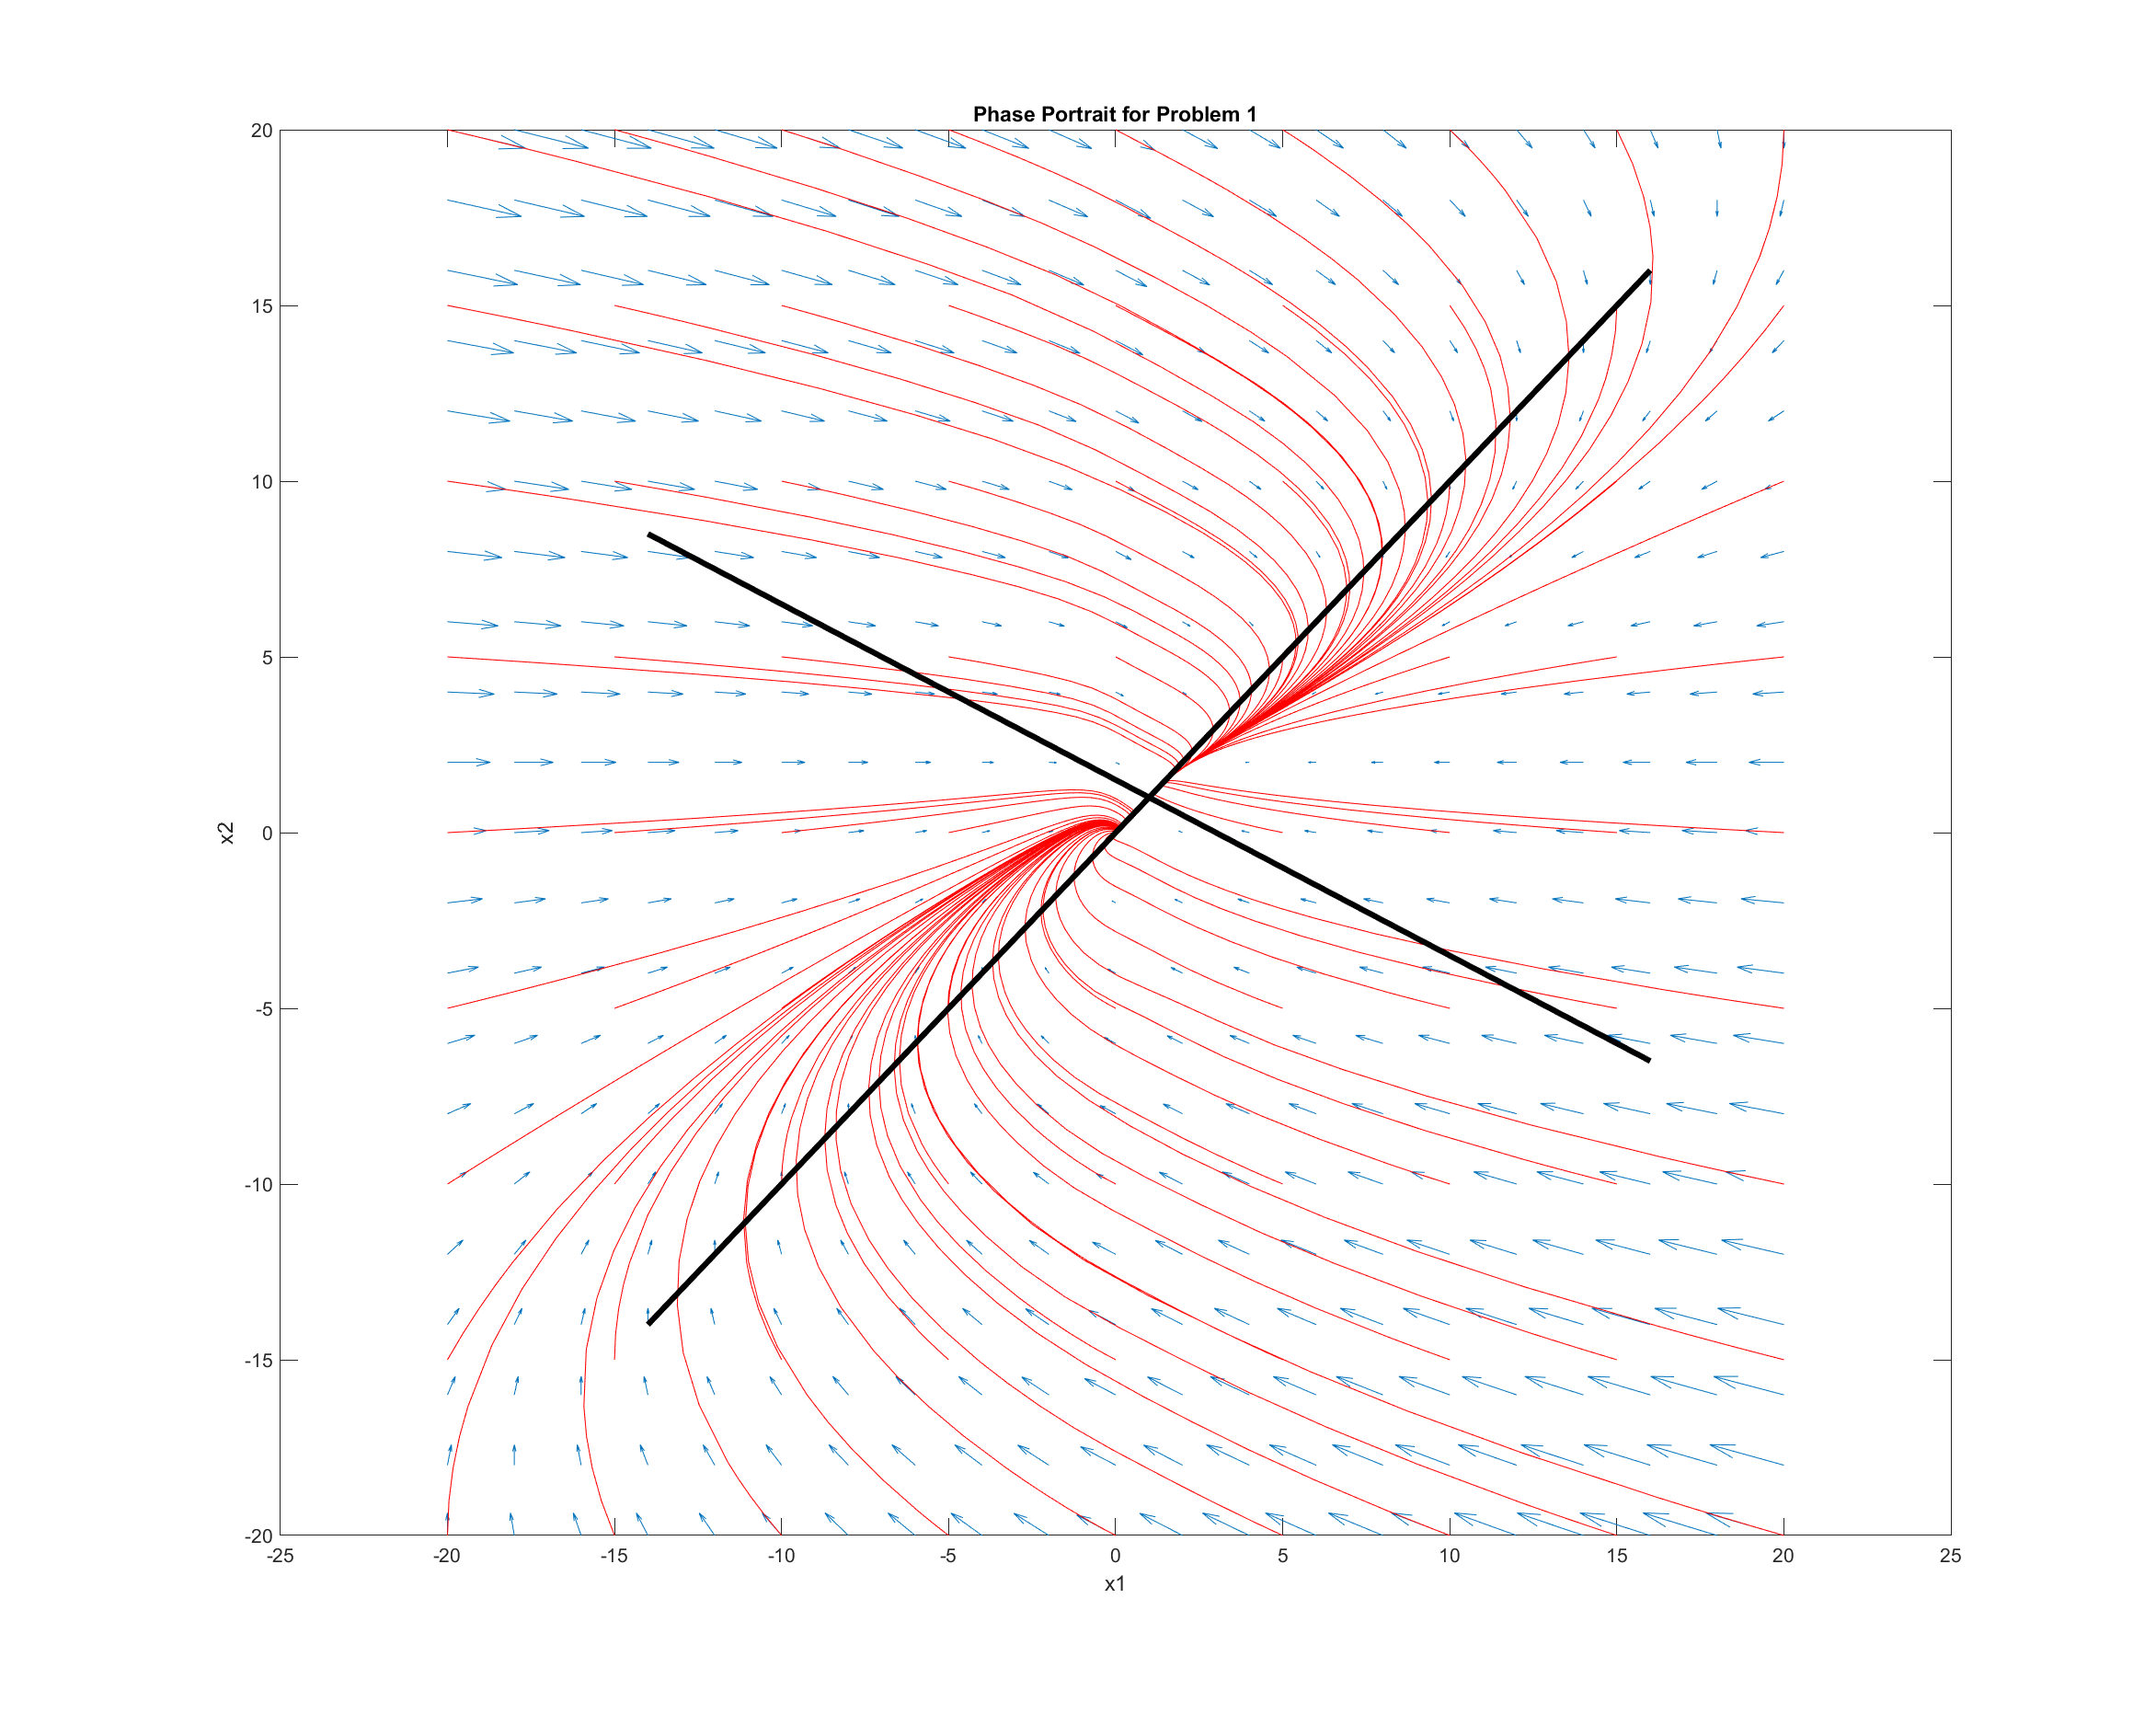
\includegraphics[width=\linewidth]{fig/pblm1}
	\caption{Phase Portrait for the original system.}
	\label{fig:pblm1}
\end{figure}


\newpage
\section{Problem 2 - S 3.7.3}
\textbf{Problem:}
A simple model of a fishery is given as
\begin{equation}
	\dot{N} = r N (1 - \frac{N}{K}) - H
\end{equation}
where $N$ represents the fish population, $H > 0$ is the number of fish harvested at a constant rate, and both $r$ and $K$ are constants.\\
Redefine the model in terms of $x$, $\tau$, and $h$. Then plot the vector field for various values of $h$. Then identify $h_c$ and classify and discuss the bifurcation.\\

\noindent
\textbf{Solution:}
\subsection{Part a}
Let $x = N / K$, this can then be substituted as
\begin{align}
	\dot{N} = \dv{N}{t} = \dv{x}{t}	
	&= r (K x) \qty(1 - x) - H\\
	\frac{1}{r K} \dv{x}{t}
	&= x \qty(1 - x) - \frac{H}{r K}
	\intertext{Let $h = \frac{H}{r K}$ and $\tau = r K t$,}
	\dv{x}{\tau} &= x (1 - x) - h
\end{align}

\newpage
\subsection{Part b}

The MATLAB code in \appendixname \ref{apx:matlab} plots a vector field of the simplified fishery model as seem in \figurename \ref{fig:pblm5}.

\begin{figure}[h]
	\centering
	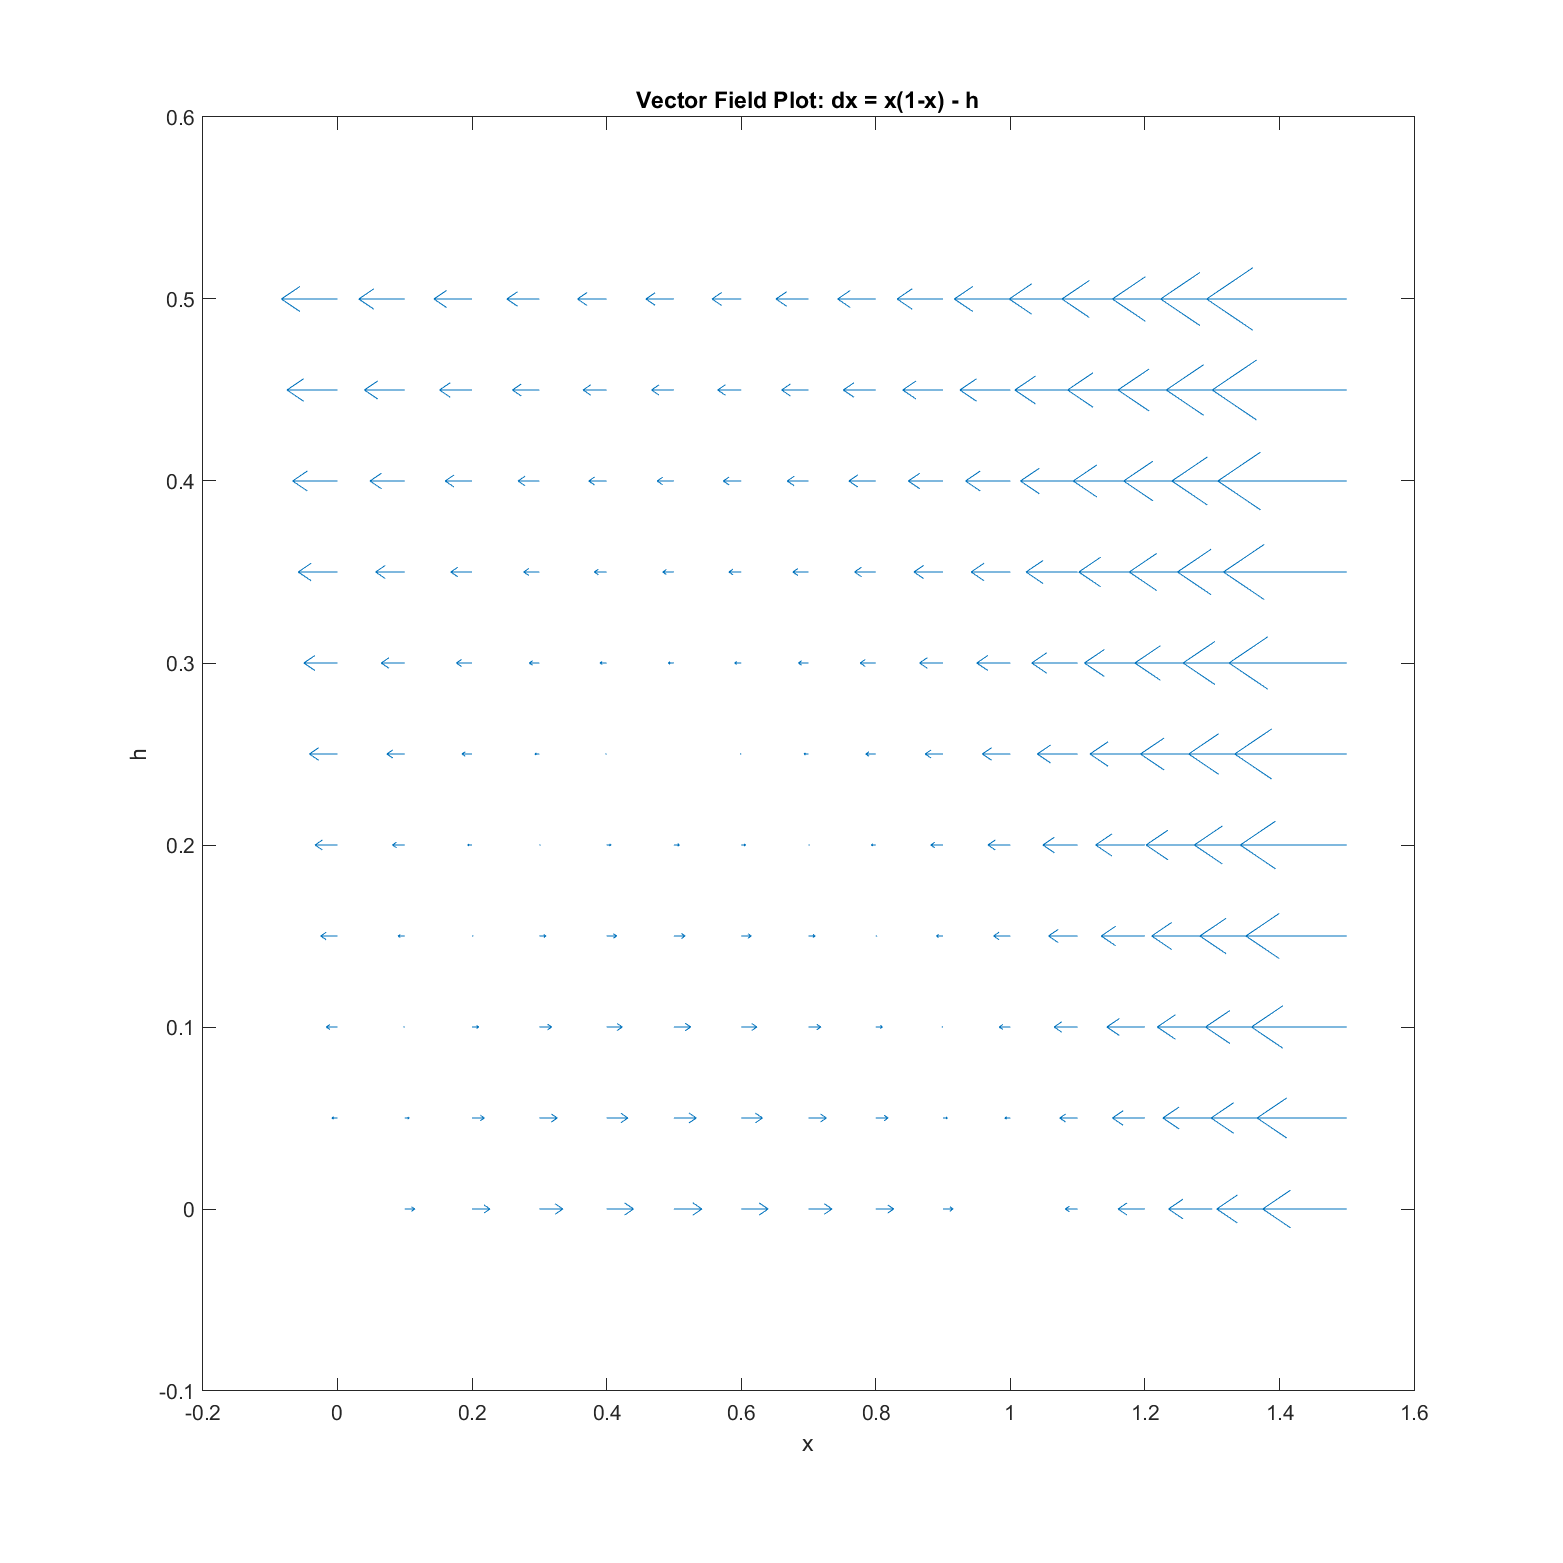
\includegraphics[width=0.7\linewidth]{fig/pblm2}
	\caption{Vector field of the simple fishery model.}
	\label{fig:pblm2}
\end{figure}

\subsection{Part c}
As is evident by observing the vector fields shown in \ref{fig:pblm2} there exists an $h_c = 0.25$ where the bifurcation occurs. This is a form of fold bifurcation.

\subsection{Part d}
The long time behavior of this model results in either a stable steady-state population of fish or the extinction of the fish. When $h<h_c$, there is a point where the fishing will balance out the reproduction of the fish, but if the original population isn't large enough they could also become extinct. When $h>h_c$ there is an issue of overfishing and the fish will always become extinct.


\newpage
\section{Problem 3 - S 3.7.4}
\textbf{Problem:}
An improved model of a fishery is given as
\begin{equation}
	\dot{N} = r N (1 - \frac{N}{K}) - H \frac{N}{A + N}
\end{equation}
where $N$ represents the fish population, $H > 0$ is the number of fish harvested at a constant rate, and both $r$, $K$, $A$ are constants.\\
Define the biological interpretation of the parameter $A$. Redefine the model in terms of $x$, $\tau$, and $h$. Find and analyze various fixed points depending on the values of $a$ and $h$. Then analyze the bifurcation that occurs when $h=a$. Then find and classify the other bifurcation that occurs at $h = \frac{1}{4} (a+1)^2$ for $a<a_c$. Finally plot the stability diagram for the system for ($a,h$).\\

\noindent
\textbf{Solution:}
\subsection{Part a}
When a population of fish is being fished, there is a portion of fish that are not possible to catch (such as eggs or fish that are too old).

\subsection{Part b}
Let $x = N / K$, this can then be substituted as
\begin{align}
	\dot{N} = \dv{N}{t} = \dv{x}{t}	
	&= r (K x) \qty(1 - x) - H\frac{K x}{A + K x}\\
	\frac{1}{r K} \dv{x}{t}
	&= x \qty(1 - x) - \frac{H}{r K}\frac{K x}{A + K x}\\
	&= x \qty(1 - x) - \frac{H}{r K}\frac{K x}{K\qty(\frac{A}{K} + x)}\\
	&= x \qty(1 - x) - \frac{H}{r K}\frac{x}{\frac{A}{K} + x}\\
	\intertext{Let $h = \frac{H}{r K}$, $\tau = r K t$, and $a = \frac{A}{K}$}
	\dv{x}{\tau} &= x (1 - x) - h \frac{x}{a + x}
\end{align}

\newpage
\subsection{Part c}
The various fixed points of different regions can be determined by solving for when $$\dv{x}{\tau} = 0$$ which can be found as the solution of 
\begin{align}
	\dv{x}{\tau} = 0
	&= x (1-x) - h \cfrac{x}{a+x}\\
	\cfrac{hx}{a+x} &= x (1-x)\\
	0 &= x^3 + (a-1) x^2 + (h-a) x\\
	&= x (x^2 + (a-1) x + (h-a))
	\end{align}
which then can be solved using the quadratic formula such that the roots are given as
\begin{equation}
	x = \qty{0, \ \cfrac{1-a}{2} \pm \sqrt{\cfrac{a^2 + 2a - 4h +1}{4}}}
\end{equation}

This solution indicates that there is a possibility of 1, 2, or 3 roots depending on the quantity: $$a^2 + 2a - 4h + 1$$ When positive there are 3 equalibrium points, if equal to zero there is two, and if negative there is only one.

\subsection{Part d}
When looking exclusively near the equilibrium point at zero, a single biforcation is evident when $h = a$. This is because the roots are found as
\begin{align}
	0 &= x \qty(x^2 + (a-1)x + (0))\\
	0 &= x^2 (x + a-1)
\end{align}
which means that there is now a double root at zero and the marginal stability is lost at that point. This is also is the boundary for trans-critical bifurcation.

\subsection{Part e}
The other bifurcation shift point occurs when
\begin{align}
	0 &= a^2 + 2a - 4h + 1\\
	4h &= a^2 + 2a + 1\\
	h &= \frac{1}{4} (a+1)^2
\end{align}
where a pitchfork bifurcation occurs.

\newpage
\subsection{Part f}

The stability diagram shown in \figurename \ref{fig:pblm3} shows 3 distinct regions, and 3 boundaries, that display different response characteristics. In the blue region there is a single real root occurring at the origin, which is the case where there is over fishing and the only stable state is extinction. In the yellow region there is are three roots that exist, one always at the origin. Above the transcritical boundary there are 3 equilibrium points, a negative one, an unstable one at the origin, and a positive stable one. In the rest of the yellow region there is a stable equilibrium point at zero, and an unstable positive equilibrium point.

\begin{figure}[h]
	\centering
	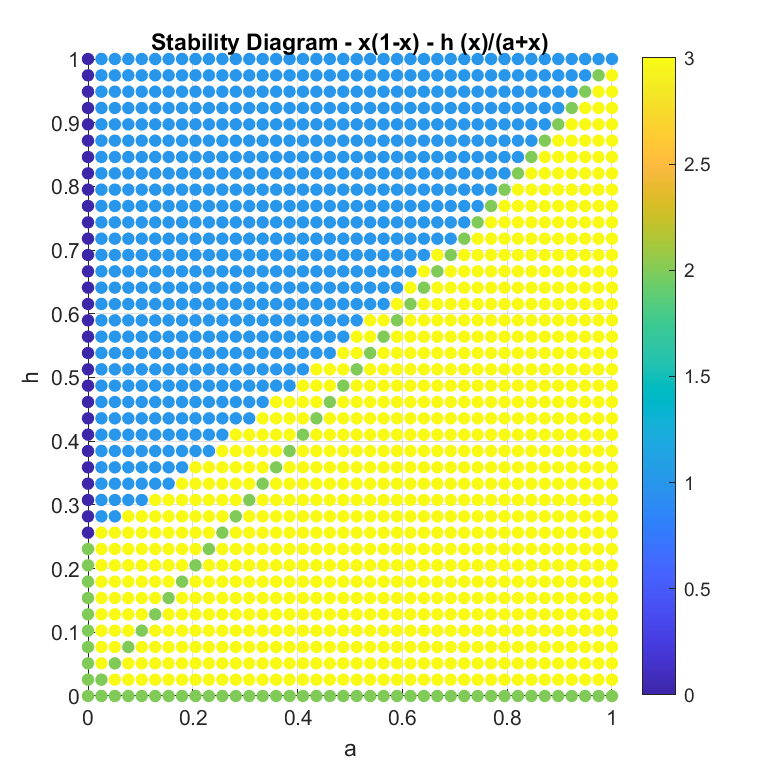
\includegraphics[width=\linewidth]{fig/pblm3}
	\caption{Stability diagram showing the roots of the system for various parameters $a$ and $h$.}
	\label{fig:pblm3}
\end{figure}




\newpage
\section{Problem 4 - K 3.8}
\textbf{Problem:}
Let the following system be defined:
\begin{equation}
	\begin{aligned}
		\dot{x}_1 &= -x_1 + \frac{2 x_2}{1 + x_2^2}, \ x_1(0) = a\\
		\dot{x}_2 &= -x_2 + \frac{2 x_1}{1 + x_1^2}, \ x_2(0) = b
	\end{aligned}
\end{equation}
Show that this system has a unique solution for all $t \geq 0$.\\

\noindent
\textbf{Solution:}

The system is known to be continuous on its domain. It is also apparent that both functions are differentiable, which results in a Jacobian of
\begin{equation}
	\mqty[-1		& \cfrac{2}{x_2^2 + 1} - \cfrac{4 x_2^2}{\qty(x_2^2 + 1)^2}\\
		  \cfrac{2}{x_1^2 + 1} - \cfrac{4 x_1^2}{\qty(x_1^2 + 1)^2} & -1]
\end{equation}
which indicates the systems dynamics are both differentiable and differential bounded. This also implies that the system is globbaly Lipshitz continuous, therefore a unique solution exists for $t\geq 0$.

\newpage
\section{Problem 5 - K 3.13}
\textbf{Problem:}
Let the following system be defined:
\begin{equation}
	\begin{aligned}
		\dot{x}_1 &= \tan^{-1}(ax_1) - x_1 x_2\\
		\dot{x}_2 &= b x_1^2 - c x_2
	\end{aligned}
\end{equation}
Derive the sensitivity equations for the parameters vary from their nominal values of $a_0 = 1$, $b_0 = 0$, and $c_0 = 1$. Then simulate the sensitivity equations and the time dependence for the initial conditions of $x_1(0) = 1$ and $x_2(0) = -1$.\\

\noindent
\textbf{Solution:}
\subsection{Part a - Sensitivity Calculation}
Let the following be defined: $$\mu = \mqty[a \\ b \\ c]$$

Let the trajectory $x(\mu, t)$ be defined with regards to parameter changes as:
\begin{equation}
	x(\mu,t) = x(\bar{\mu},t) + \eval{\pdv{x}{\mu}}_{\bar{\mu}} \tilde{\mu}
\end{equation}
where $\tilde{\mu} = \mu - \bar{\mu}$.

It can also be defined by its nonlinear definition as:
\begin{align}
	x(\mu,t) &= x_0 + \int_0^t \dot{x}(x(\mu,\tau), \mu, \tau) \dd{\tau}
	\intertext{The sensativity to the parameters can then be formulated}
	S(t) = \pdv{x}{\mu} &= 0 + \pdv{\mu} \int_0^t f(x(\mu,\tau), \mu, \tau) \dd{\tau}\\
	&=  \int_0^t \pdv{\mu} f(x(\mu,\tau), \mu, \tau) \dd{\tau}\\
	&=  \int_0^t \pdv{f}{x}\pdv{x}{\mu} \pdv{f}{\mu} \dd{\tau}
	\intertext{which can be clculated as jacobians of $f$ resulting in}
	S(t) &=  \int_0^t A(\tau) S(\tau) + B(\tau) \dd{\tau}
\end{align}
where the matrices $A(\tau)$ and $B(\tau)$ are the Jacobians with respect to $x$ and $\mu$ respectively:
\begin{align}
	A(\tau) &= \eval{\pdv{f}{x}}_{\bar{\mu}}  &B(\tau) &= \eval{\pdv{f}{\mu}}_{\bar{\mu}}\nonumber\\
			&= \mqty[-x_2 + \cfrac{x_1}{x_1^2 + 1} 	& - x_1\\
					 0								&1] &
			&= \mqty[\cfrac{x_1}{x_1^2 + 1} & 0 	& 0\\
					 0						& x_1^2 & -x_2]
\end{align}

Finally, the evolution of sensitivity over time can be found using the Leibnitz Formula, resulting in
\begin{equation}
	\dv{s(t)}{t} = A(t) S(t) + B(t)
\end{equation}

\subsection{Part b - Simulation}
The MATLAB code in \appendixname \ref{apx:matlab} simulates and plots the states and sensitivities for each of the parameters. These plots can be seen in \figurename \ref{fig:pblm5}.

\begin{figure}[h]
	\centering
	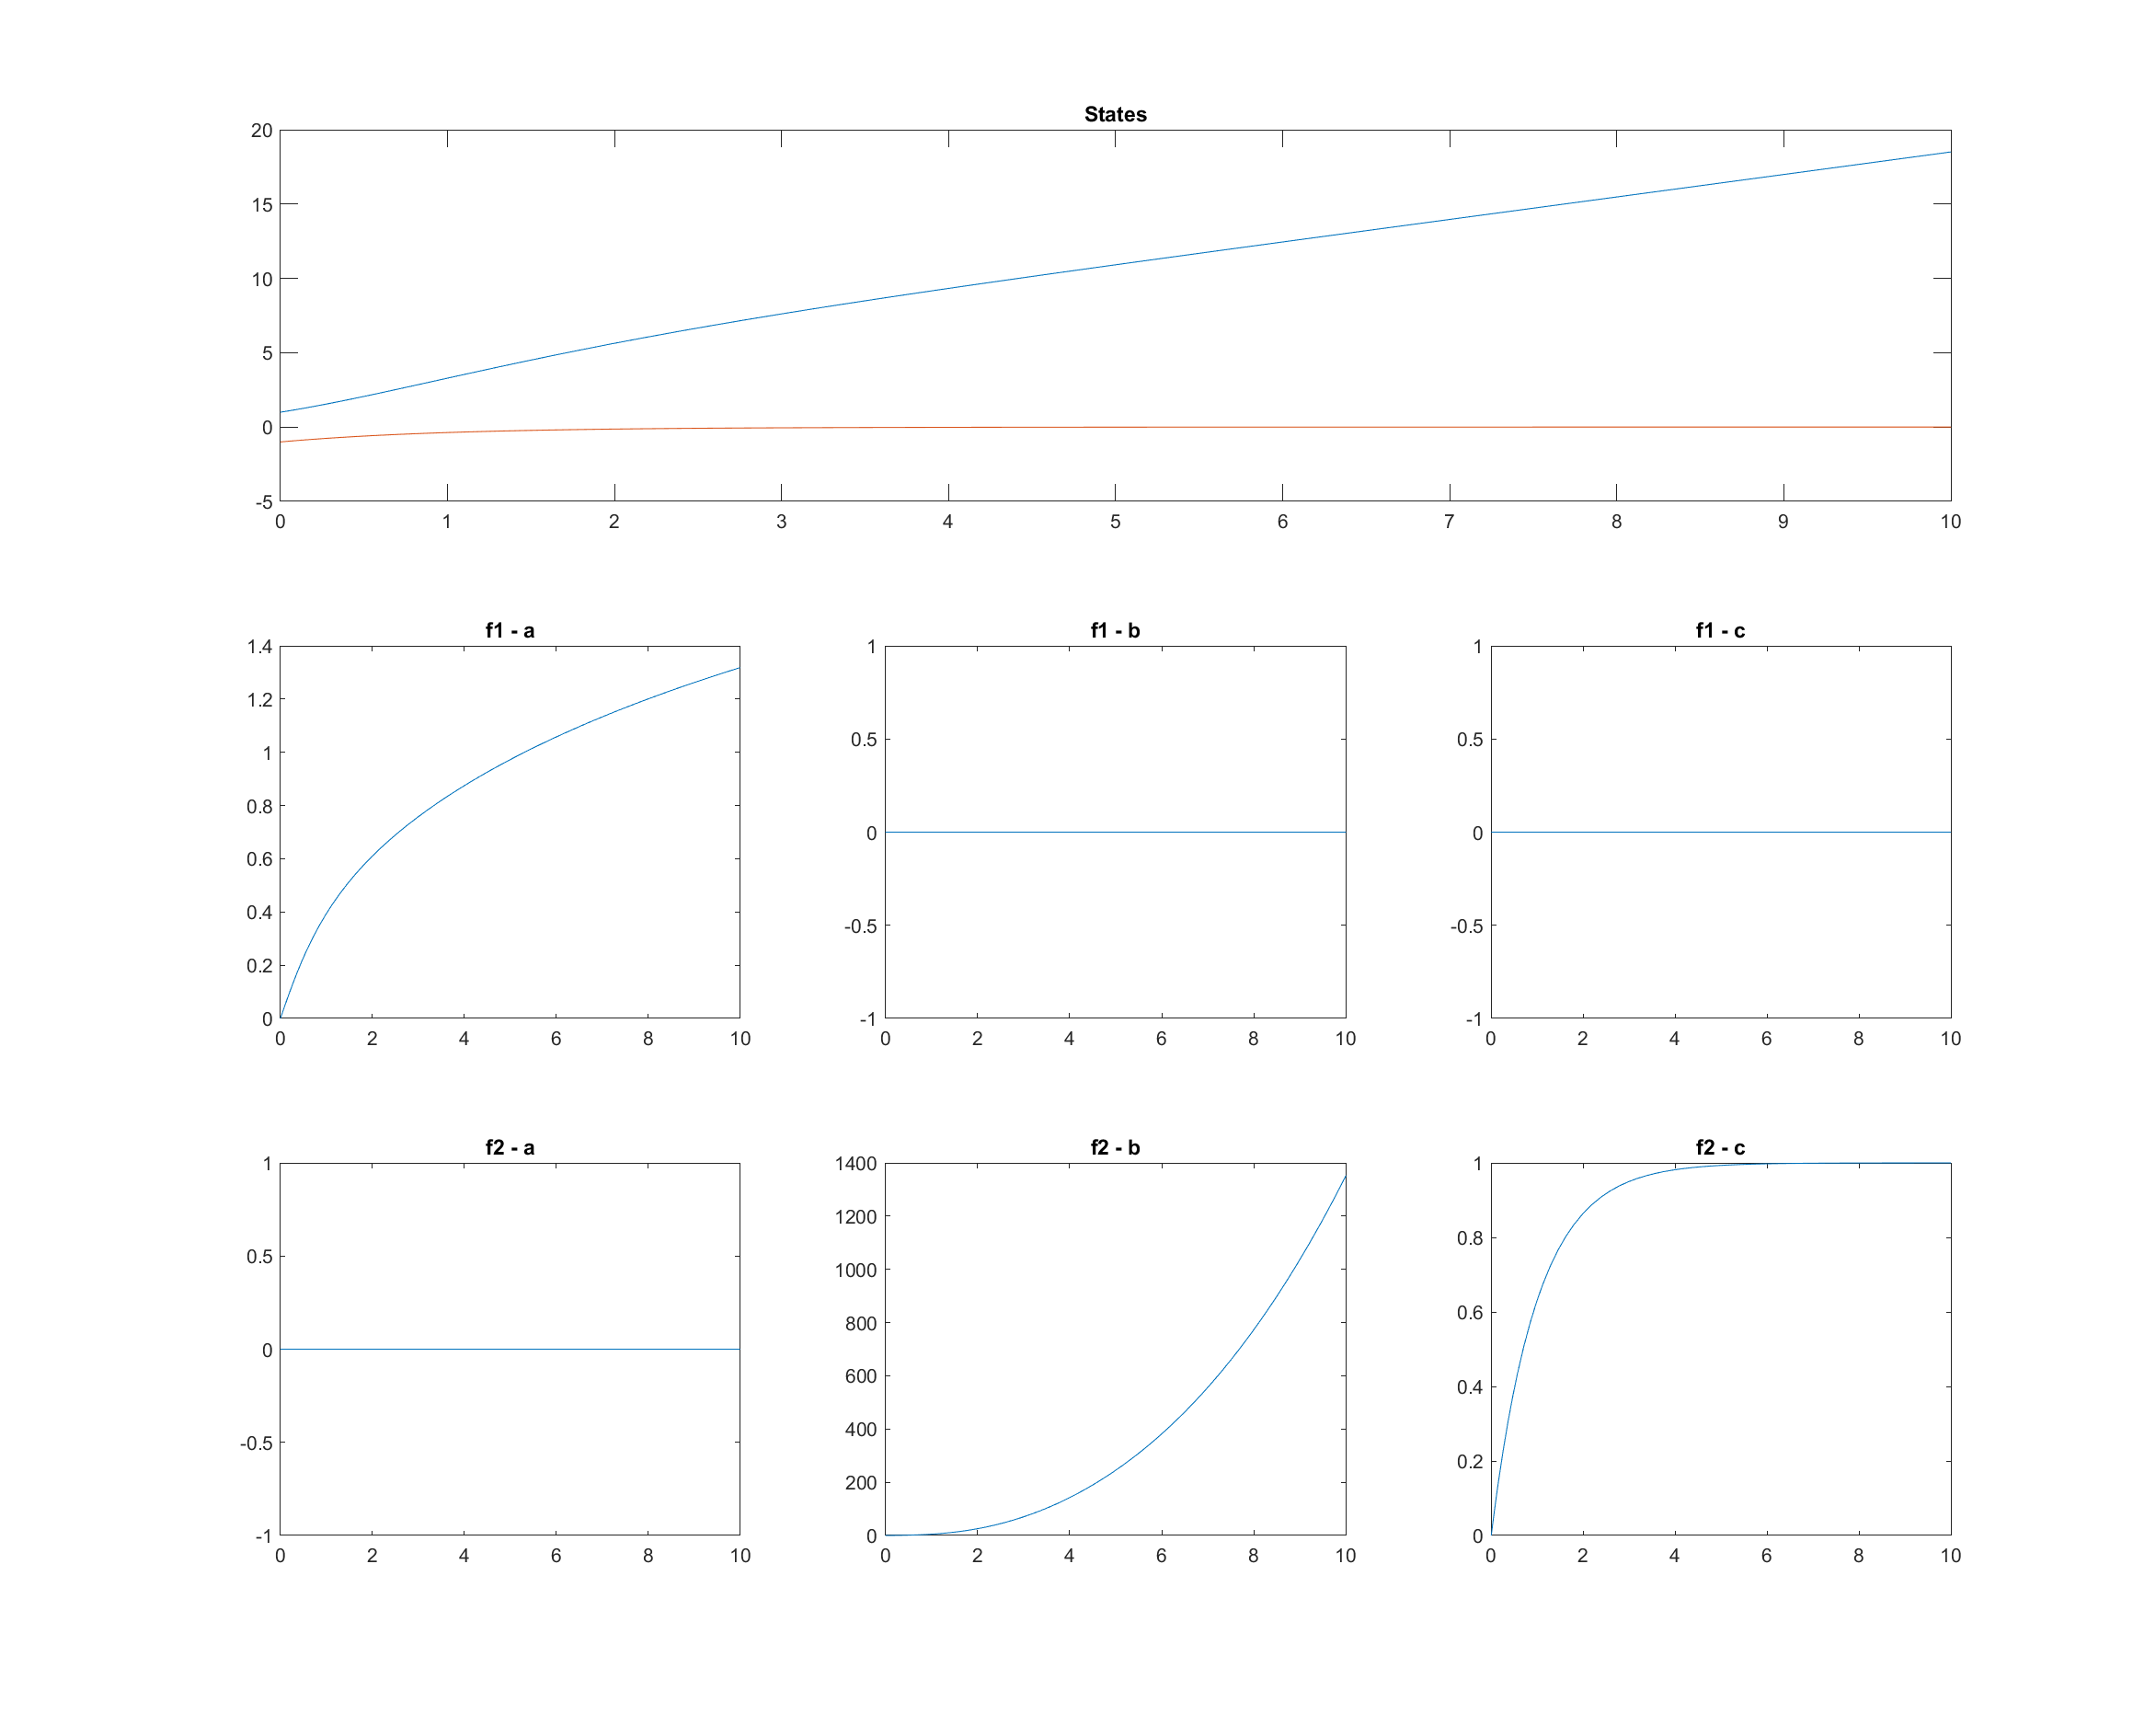
\includegraphics[width=\linewidth]{fig/pblm5}
	\caption{Simulation for Problem 5 with the evolution of sensitivities to parameters.}
	\label{fig:pblm5}
\end{figure}

\newpage
\appendix
\section{MATLAB Code:}\label{apx:matlab}
All code I write in this course can be found on my GitHub repository:\\
\href{https://github.com/jonaswagner2826/MECH6313}{https://github.com/jonaswagner2826/MECH6313}
% MECH6313_HW3
\lstinputlisting[caption={MECH6313\_HW3},label={script:HW1}]{MECH6313_HW3.m}


\end{document}
